\section{Overview of Interaction Theorem Proving (ITP) Systems}
\label{sec:overview}

This section provides a brief overview of the ITP systems in terms of their major distinguishing characteristics followed by a detailed comparison of a small set of representative systems. Although the focus of this survey is not on the formal logic underlying the proof assistants, to understand the difference among them as well as the techniques from the literature described in later sections, we need to talk about theories at least to some extent. In fact, salient characteristics that distinguish different ITP systems boost from the formal foundations they are based on. In the following, these ITP systems are introduced as they historically emerged following the development of the different formal foundations of mathematics informing readers to both simultaneously. % in an attempt to familiarize readers simultaneously to both.

The first attempt in mechanical verification of mathematical proofs is the Automath~\cite{Bruijn_1983} system, initiated by De Bruijn in 1967. It treats proof as a first-class object like any other term in formal language. This technique, in logic, is known as Curry-Howard-Isomorphism that states one-to-one correspondence between formal proof calculi and type systems for a model of computation, e.g., between natural deduction and typed system for lambda calculus. %This correspondence, in fact, splits into two - formula_as_types and proof_as_programs. 
Martin-L{\"o}f’s Intuitionistic Theory of Types~\cite{Lof_1984} extends the Curry-Howard-Isomorphism to predicate logic by introducing dependent types and then later, after the discovery of Girad's paradox, replaced the original impredicative version with a consistent predicative version. There are both extensional and intensional variants of this type theory, which are implemented in proof assistants Nuprl and Agda, respectively. I'll explain both predicativity and intensionality later in the section. 

On the other hand, under Curry-Howard-Isomorphism, Girad's polymorphic $\lambda$-calculus, system F\_$\omega$, corresponds to higher-order logic. Theory Coquand, in 1985, combined system F\_$\omega$ with impredicative Martin-L{\"o}f type theory in a higher-order extension of Automath language and presented Calculus of Constructions (CoC)~\cite{Coquand_Huet_1988}. CoC was later extended with primitive inductive extension leading to the Calculus of Inductive Constructions (CIC). The proof assistant, Coq, is the implementation of this calculus. The current Coq system's logic is dependently typed, higher-order, partially predicative, and intensional~\cite{Coq_2019}.

Automath also initiated the concept of Logical Framework. De Bruijn's systems only give basic mathematical mechanisms and let the user implement their preferred logical rules. Thus, in a logical framework, one can embed a logic as a signature in the framework's type theory, and the provability of a formula in the embedded logic comes down to the type inhabitation problem of the framework's type theory. Systems LF, Twelf are some implementations of Logical framework. Around the same time as Automath, another deductive system, the logic of computable functions was devised by Dana Scott~\cite{Scott_1993} and later, implemented in an ITP system, called Logic for Computable Functions (LCF), by Robin Milner and his collaborators at Stanford, Edinburgh, and Cambridge. Milner later developed the \emph{LCF approach} for his systems to not to require storing and rechecking of large proof objects~\cite{Geuvers_2009}. This LCF approach provides soundness by construction by making proofs terms of an abstract data type \emph{thm} whose predefined values are axioms and constructors are primitive inference rules of the logic. One can only create a term of \emph{thm} via the inference rules; thus, the proof has to be sound. Several present ITP systems, including as Isabelle~\cite{Wenzel_2008}, HOL~\cite{Gordon_Melham_1993}, and HOL-Light, are successors of LCF system. Isabelle, in fact, is an LCF style logical framework with the logic directly encoded in LCF style serving as meta-logic for other logic to be embedded as object logic. Examples of embedding are Isabelle/HOL and Isabelle/ZF, where HOL is classical higher-order object logic, and ZF stands for first-order Zermelo-Frankel set theory. 

There are few other active ITP systems that have not been mentioned above. Among them, Mizar is quite notable for its largest repository of formalized mathematics called the Mizar Mathematical Library (MML). Mizar's other famous and influential feature is its declarative input language, which enables batch proof checking. It can check a whole file at once even if there are some proof steps not acceptable by the solver, consequently creating a syntactically correct proof with potential holes in it. The precise notion of this method can be found in Wiedijk's work~\cite{Wiedijk_2003_b}. This feature, named Mizar Mode, has been incorporated in many proof assistants, including HOL, HOL Light, Isabelle, Coq~\cite{Geuvers_2009, ringer_et_al_2019_b}. A complete overview of all other ITP systems such as LEGO, Lean, Idris can be found in~\cite{Wiedijk_2003_a, Harrison_2014, Geuvers_2009}.

\subsection{Detailed Comparison of a Few ITP Systems}

For the detailed comparison, I have selected the representative systems Coq, Agda, Nuprl, Isabelle/HOL in the attempt to cover most formal systems and their branches. They are compared based on the following categories that have practical implications on proof development. \\

%to represent systems based on impredicative Calculus of Inductive Construction, Predicative Martin-L{\"o}f intensional, Predicative Martin-L{\"o}f extensional, intensional  

\textbf{Equality}
The definition of \emph{equality} in type theory has great implication on proof development and type checking in the corresponding proof assistant. Extensional and intensional type theories handle \emph{equality} differently. Extensional equality considers two objects to be equal if their external properties are alike i.e., they behave the same way with its environment. Intensional equality, on the other hand, requires the internal structure of the entities to be equal as well. For example, $f(n) = 3*n + 9$ and $g(n) = 3 * (n+3)$ are equal in extensional sense but not, in intensional sense. Similarly, two functions are considered equal by extensionality, known as \emph{function extensionality} if they produce same outputs for the same inputs, where in intensionality, their implementation needs to same as well. Therefore, in proof assistants, based on intensional type theory such as Coq, Agda, if inductive definition of plus (+) defines $0 + n = n$ but not $n + 0 = n$, then any statement of the later construct needs additional induction reasoning to hold i.e. needs to be proved. On the other hand, in extensional type theory based proof assistants such as Nuprl,type checking is undecidable. The reason is in extensional type theory, \emph{definitional equality} that refers to equality by construction, and \emph{propositional equality}, used in propositional statements to be proved, coincide. Consequently, undecidable programs can be specified in the type system making type checking undecidable. However, in intensional type theory \emph{definitional equality} and \emph{propositional equality} are completely distinct, and type checking is decidable. \\

\textbf{De Bruijn Criterion} 
De Bruijn Criterion~\cite{Barendregt_Geuvers_2001} requires proof assistants to produce an independently checkable proof object for the interactively created proof in the system. This proof object should be easily verified by skeptic users by writing a simple type checking algorithm. This is one of the four ways identified by H. Guevers~\cite{Geuvers_2009} to guarantee the correctness of ITP systems. Coq, Agda, Nuprl all meet the De Bruijn criterion. However, systems based on LCF, such as Isabelle, do not produce a complete proof object as each step is constructed with the guarantee that it is correct. In that sense, they do not meet the \emph{De Bruijn criterion} though it should not be hard to generate a proof object on the side if needed. The practical implication is that, in the LCF approach, there is no need to check the system with respect to the theory anymore as its inference rules and axioms are implemented directly to create the proof. \\

\textbf{Predicativity}
Predicativity of type theory has impact on its consistency as well as on its expressiveness. Impredicative refers to self-referential definition i.e., a definition that mentions or quantifies over itself. To be predicative, a definition can not mention itself, and if it contains quantifiers, then they can not be initiated with an object defined by the definition. Impredicative type system can be shown inconsistent by Girad's paradox thus Martin-L{\"o}f made his type theory predicative. Agda, Nuprl, meta-logic in Isabelle, all are predicative. However, in Coq, Type universe, including Set is predicative, but the Prop universe is still impredicative due to the informally agreed notion that it is often easier to express mathematical proofs with impredicativity. \\

\textbf{Termination and Totality}
In proof assistants based on intuitionistic type theories such as Coq, Agda, and Nuprl, functions need to be terminating for the logic to be consistent. Recursive calls have to be made on the subterm of the arguments to ensure their termination. For advanced cases where termination cannot be proven automatically, explicit proof of termination needs to be provided, or special approaches like exploiting the size of argument terms~\cite{Abel_et_al_2017, Ringer_et_al_2019} needs to be used. Agda provides induction-recursion that lets the user define mutually recursive functions and data types. Coq does not have this mechanism. However, classical higher-order logic in HOL, do not need a termination witness, but the use of the non-terminating function is limited~\cite{Ringer_et_al_2019}. Moreover, functions in HOL and CIC logic need to total, and partial function needs indirect encoding into the logic. These requirements are two difficulties beginners in ITP usually encounter, even if they are already familiar with functional programming language~\cite{Ringer_et_al_2019}. \\
%total partial~\cite{McBride 2015, Capretta, V. 2005, Bertot and Casteran, 2004, Ringer}

\textbf{Proof Creation Style}
Proof creation style varies widely among ITP systems. In Coq, although it supports forward style, the usual way to create a proof is to use backward style (top-down). The user keeps applying tactics to the current goal, which creates subgoals needed to be proven separately, until True is reached. Proof development in Nuprl also follows the top-down approach. However, in Isabelle, the usual way is the forward style (bottom-up), where proofs are created from axioms and inference rules from the logic. Proof context gets enriched by new facts keeping the goal same, until the goal is reached~\cite{Yushkovskiy_Tripakis_2018}. However, both of them support tactics and provide tactic languages Ltac and Eisbach, respectively, to allow writing custom tactics. They also have proof languages like Coq/SSReflect and Isabelle/Isar. Proof languages aid in writing understandable proofs inspired by mathematical vernacular, in contrast to unstructured sequences of tactics. Users can reconstruct an English proof just form the script of the proof instead of stepping through tactics and tracking goal transformation. 

However, in Agda, there is no support for the separate tactic language, although an automatic proof search tool, Agsy that works like \emph{auto} tactic in Coq is there. Agda's dependent types let the user write almost any proposition. Proofs can be written as the term of the type of its theorem proposition. However, users can build proofs interactively in Emacs or atoms by putting a question mark (?) in the place of an expression, usually the proof term they need to write. Agda is able to type check incomplete programs with holes, i.e. (?) marks and can provide a list of the context, infer the type of the expression at the hole, and even sometimes evaluate the open term if bound variables in surrounding context are provided. Agda, like Idris, is basically a dependently typed programming language whose type storing and dependent types let it act as a proof assistant. The syntax in Agda is Haskell like where Coq's syntax is ML like. \\

\textbf{Dependent Types and Pattern Matching on them} 
Coq, Agda, and Nuprl support dependent types, but Isabelle/HOL does not have dependent types. However, it is easier to pattern match on dependent types in Agda than in Coq. In coq, one needs to use complex clause like \emph{match.....as.....return} clauses for that. Examples of pattern matching on indexed datatypes in Coq and Agda are shown side by side in the following Fig~\ref{fig:overview_1}.  \\


\begin{figure}[H]
	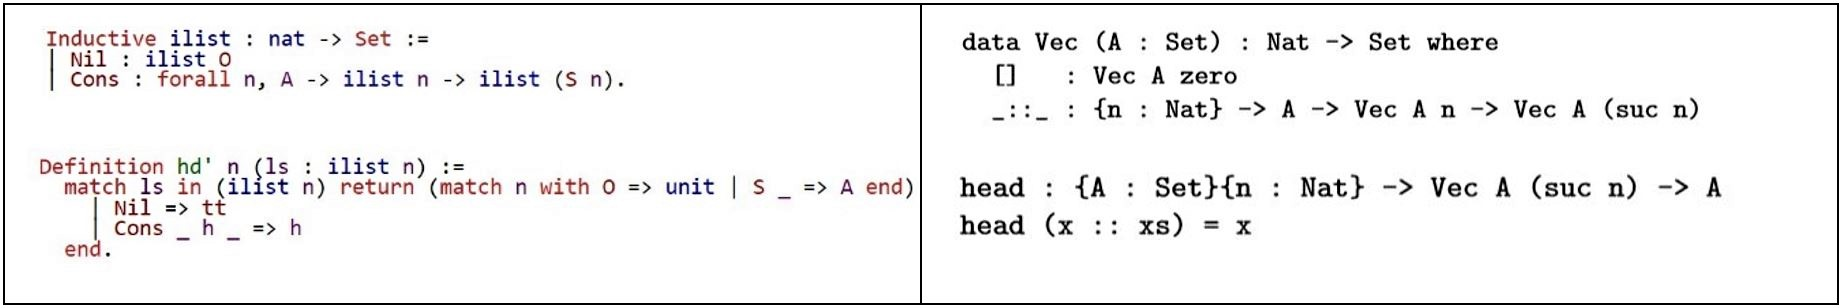
\includegraphics[width=15cm]{figures/fig_1.JPG}
	\centering
	\caption{Pattern matching on indexed data-types in Coq and Agda respectively~\cite{Chlipala_CPDT_2013}~\cite{Norell_2009}}
	\label{fig:overview_1}
\end{figure}


\textbf{Program Extraction}
Program extraction from proofs let certified program to be extracted and executed in favorable run-time environment.This mechanism is beneficial for system verification projects. Coq supports the extraction of executable programs in Ocaml and Haskell from proofs. Agda does not have any such support at this moment. Isabelle/HOL also has a code generation scheme based on the work of Haftmann and Nipkow~\cite{Haftmann_Nipkow_2010}. It translates HOL to an intermediate language called Mini-Haskell and then, translates from this Mini-Haskell to Ocaml, Haskell or Standard ML. \\

\textbf{Classical axioms}
Classical axioms cannot be proved in all proof assistants because of their underlying logic, thus require special techniques when they are needed in proof development but not supported by the ITP systems. Isabelle/HOL is based on classical higher-order logic. Hence, all classical axioms, e.g., Excluded middle, Double negations, are valid here. However, in intuitionistic logic, not all of them hold. For example, the double negation introduction law can be easily proven in intuitionistic logic, but neither the double negation elimination rule nor the Excluded middle can be proven. One way to embed Excluded middle axiom into intuitionistic logic is by double negating it, which is known as Glivenko's double-negation translation. Other classical axioms can also be translated through various translations such as Kudro's translation, G{\"o}del-Gentzen translation~\cite{Yushkovskiy_Tripakis_2018}. Coq provides a library, Coq.Logic.Classical\_Prop with classical axioms, to extend its intuitionistic logic to classical logic. 













